%-------------------------------------------------
\documentclass[tk,diplom]{daposterifn}
%-------------------------------------------------
%* options:
%* tnt, hf, tk, mns /default: -none-
%* diplom, master   /default: diplom
%* extern


%-------------------------------------------------
% BITTE HIER PARAMETER SETZEN!
%-------------------------------------------------

\setDAParameter[\LARGE]{Thema}{Compressed Compute-and-Forward mit korrelierten Audiosignalen}
\setDAParameter{Student}{Florian Roth, Raphael Hildebrand, Lucas Weber, Orell Garten}
\setDAParameter{BetreuerTUD}{Dipl.-Ing. Carsten Herrmann}
%\setDAParameter{BetreuerExternName}{}
%\setDAParameter{BetreuerExternFirma}{}
\setDAParameter{Hochschullehrer}{Prof. Dr.-Ing. Frank Fitzek}
\setDAParameter{VerteidigungDatum}{11.08.2016}

%-------------------------------------------------

% \setStudentPassbild[5.0cm]{./figures/passbild}
% \setStudentWerdegang[\small][1.0ex]{%
% 	07/2003\newline
% 	Schulabschluss in Sowieso-Dingskirchen
% 	
% %	seit 10/2003\newline
% %	Studium Elektrotechnik an der TU Bergakademie Freiberg
% 	
% 	seit 10/2005\newline
% 	Studium Elektrotechnik, Studienrichtung Informationstechnik, an der TU Dresden
% 	
% %	10/2007 - 03/2008\newline
% %	Auslandsstudium an der �cole Polytechnique F�d�rale de Lausanne, Schweiz
% 	
% 	10/2008 - 03/2009\newline
% 	Fachpraktikum bei Firma-Fiktiv und Partner in GanzWoAnders-Blahausen
% }


%-------------------------------------------------
% BEGINN DES DOKUMENTS
%-------------------------------------------------

\begin{document}


\includeDADetails


%* uncomment next line to switch the document language (for caption labels etc.) to English (default: German)
%\selectlanguage{english}


\begin{multicols}{3}


%-------------------------------------------------
% BITTE HIER EIGENEN INHALT EINF�GEN!
%-------------------------------------------------

%-------------------------------------------------
\section*{Einleitung}
%-------------------------------------------------

Im Jahr 2022 werden �ber 500 Millionen im Internet aktive Ger�te erwartet. Diese erzeugen eine gro�e Masse an Daten, die �ber das Netzwerk transportiert werden m�ssen. Dies muss zuverl�ssig und m�glichst schnell passieren. Idealerweise verbrauche alle beteiligten Ger�te au�erdem sehr wenig Energie. Zur guten Erfassung der Umgebung werden in bestimmten Szenarien massenhafte Sensoren ben�tigt. Damit verbunden sind gro�er Herausforderungen bez�glich der Netzwerkkapazit�t, da viele Sensoren auch enorm viele Daten generieren. In vielen Situationen, sind die Datenstr�me der unterschiedlichen Sensoren jedoch miteinander korreliert, sodass sich diese Korrelation ausnutzen l�sst, um die Datenmenge im Netzwerk zu verringern. Unsere Arbeit bietet hier eine M�glichkeit Signale bez�glich ihrer Korrelation zu klassifizieren. 


%-------------------------------------------------
\section*{Theoretische Vorbetrachtung}
%-------------------------------------------------

Lorem ipsum dolor sit amet, consectetuer adipiscing elit, sed diam nonummy nibh euismod tincidunt ut laoreet dolore magna aliquam erat volutpat. Ut wisi enim ad minim veniam, quis nostrud exerci tation ullamcorper suscipit lobortis nisl ut aliquip ex ea commodo consequat.


%-------------------------------------------------
\subsection*{Kennwerte}

Lorem ipsum dolor sit amet, consectetuer adipiscing elit, sed diam nonummy nibh euismod tincidunt ut laoreet dolore magna aliquam erat volutpat. Ut wisi enim ad minim veniam $c = \sqrt{a^2 + b^2}$, quis nostrud exerci tation ullamcorper suscipit lobortis nisl ut aliquip ex ea commodo consequat.
\begin{alignat*}{1}
	y = \sum_{i=1}^{M} \left[ c_i \, \frac{x_i - \alpha}{1 + \prod_{j=1}^{M} r_{i,j} x_i} + \max \{ \theta_i, \sigma^2 \} \right]
\end{alignat*}
Lorem ipsum dolor sit amet, consectetuer adipiscing elit, sed diam nonummy nibh euismod tincidunt ut laoreet dolore magna aliquam erat volutpat.

Ut wisi enim ad minim veniam, quis nostrud exerci tation ullamcorper suscipit lobortis nisl ut aliquip ex ea commodo consequat.


%-------------------------------------------------
\section*{Octave-Programm}
%-------------------------------------------------

Die im vorherigen Abschnitt vorgestellen Ma�zahlen wurden im n�chsten Schritt in einem Octave-Skript implementiert. Das Programm besteht aus 3 funktionalen Einheiten: Automatisches Einlesen der Audiodateien, Berechnung der Korrelation und der Kennwerte und dem Speichern der errechneten Werte in einer Exceldatei. Im Quellcode selbst k�nnen bestimmte Parameter eingestellt werden, die die Berechnung auf verschiedenste Weise beeinflussen. Besonders zu bemerken ist, dass man beliebige Abschnitte des Signals systematisch korrelieren kann, so dass man aus wenigen Signalen bereits sehr viele Werte bekommen kann. Die genutzen Abschnitte werden wiederum als extra .wav-Datei gespeichert.\\ Das Skript ist modular aufgebaut, so dass es vergleichsweise einfach m�glich weitere Analysemethoden zu entwickeln und zu implementieren. Zuk�nftig w�re es au�erdem sinnvoll die Berechnung der Korrelationen zu parallelisieren und so die Ausf�hrung des Programms wesentlich zu beschleunigen. 

%-------------------------------------------------
\subsection*{Ablaufplan}

Prinzipskizze des Programmablaufs

\begin{center}
	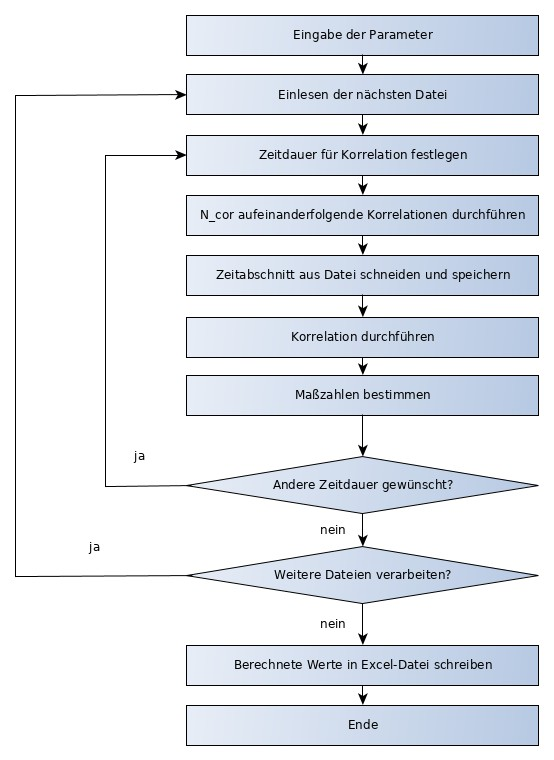
\includegraphics[width=\linewidth]{./img/pap}
	\captionof{figure}{Programmablaufplan\label{fig:Programmablauf}}
\end{center}


\begin{center}
	\begin{tabularx}{\linewidth}{|l|X|X|}
	  \hline
		jdffdslf & fjdsf jhg lkjgljfdlg jfdj jrgjfdkgeag & jfdfjwgr igjirejg \\ \hline
		ejperg   & jgjk rpe jbhpets jpgfg                & gkfdl gh jthjp trhks tpsjrst�j trjs js irithjmn \\ \hline
	\end{tabularx}
	\captionof{table}{Unterschrift f�r Tabelle.\label{tab:tabelle}}
\end{center}

\blindtext[1]

%-------------------------------------------------
\section*{Signalauswahl}
%-------------------------------------------------

Lorem ipsum dolor sit amet, consectetuer adipiscing elit, sed diam nonummy nibh euismod tincidunt ut laoreet dolore magna aliquam erat volutpat. Ut wisi enim ad minim veniam, quis nostrud exerci tation ullamcorper suscipit lobortis nisl ut aliquip ex ea commodo consequat.

Donec fringilla rhoncus dolor et pretium. Donec non neque eget mi imperdiet porttitor. Nulla facilisi. Ut porta justo nec tortor sollicitudin in elementum sem lobortis. Sed non cursus nunc. Morbi ac felis mollis dolor pulvinar ullamcorper id nec dui. Sed id nibh magna, sit amet laoreet elit.
\begin{enumerate}
	\item Duis adipiscing venenatis risus, et condimentum risus commodo nec.
	\item Quisque ut leo quis leo porta pellentesque ut sit amet leo. Phasellus quis pharetra nisl.
	\item Fusce imperdiet rhoncus ante, sed iaculis elit euismod vel.
\end{enumerate}
Aenean ac nulla ipsum. Sed nulla dui, consectetur sit amet ultrices eget, semper nec ipsum. Pellentesque lacinia ornare sapien, ac accumsan nulla congue eget. Aliquam gravida nulla id justo egestas accumsan.

Vestibulum convallis malesuada faucibus. Vestibulum ligula turpis, venenatis vel gravida at, eleifend eget tortor. Phasellus blandit nisi vel leo euismod a vestibulum est vestibulum. Duis convallis dignissim turpis. Nam ullamcorper molestie urna et iaculis.

\blindtext[1]

\subsection*{Beispielsignal}
Vestibulum convallis malesuada faucibus. Vestibulum ligula turpis, venenatis vel gravida at, eleifend eget tortor. Phasellus blandit nisi vel leo euismod a vestibulum est vestibulum. Duis convallis dignissim turpis. Nam ullamcorper molestie urna et iaculis.

%-------------------------------------------------
\section*{Zusammenfassung}
%-------------------------------------------------

In dieser Arbeit wurden Modelle entwickelt, die die Korrelation der beiden Audio-Kan�le einer Stereoaufnahme bez�glich ihres Abklingverhaltens und dominierenden Anteilen beschreiben. Diese Modelle wurden als Grundlage f�r die Entwicklung eines Octave-Skripts genutzt, welches eine massenhafte Klassifizierung von Audiodaten bez�glich der entwickelten Kriterien erm�glicht. Abschlie�end wurden Testsignale aufgenommen. \newline In Zukunft m�ssen die Modelle entsprechend der genauen Anwendung weiter entwickelt werden.



\end{multicols}


\end{document}
